\documentclass[11pt,a4paper]{article}

\usepackage[utf8]{inputenc}
\usepackage[T1]{fontenc}
\usepackage{amsmath,amssymb,amsthm}
\usepackage{mathtools}
\usepackage{geometry}
\usepackage{tikz}
\usepackage{pgfplots}
\usepackage{hyperref}
\usepackage{enumitem}
\usepackage{booktabs}
\usepackage{xcolor}
\usepackage{microtype}
\usepackage{titlesec}

\geometry{margin=1in}
\pgfplotsset{compat=1.18}
\usetikzlibrary{arrows.meta,calc,positioning}

\definecolor{accent}{HTML}{e8624a}
\definecolor{accentblue}{HTML}{5b8dee}
\definecolor{accentgreen}{HTML}{2f9e72}
\definecolor{gold}{HTML}{c58b22}
\definecolor{mutedtext}{HTML}{6f6b7d}

\newtheorem{theorem}{Theorem}[section]
\newtheorem{proposition}[theorem]{Proposition}
\newtheorem{corollary}[theorem]{Corollary}
\newtheorem{lemma}[theorem]{Lemma}
\theoremstyle{definition}
\newtheorem{definition}[theorem]{Definition}
\newtheorem{example}[theorem]{Example}
\theoremstyle{remark}
\newtheorem{remark}[theorem]{Remark}

\newcommand{\supp}{\operatorname{supp}}
\newcommand{\KL}{D_{\mathrm{KL}}}
\newcommand{\simplex}{\Delta(\mathcal X)}

\hypersetup{
  colorlinks=true,
  linkcolor=accent,
  citecolor=accentblue,
  urlcolor=accentblue
}

\title{%
  \vspace{-1cm}
  {\Large\scshape Support Singularities and Softmax Geometry}\\[0.6em]
  \textbf{What Cross-Entropy Does---and Does Not---Diverge On}
}
\author{Taha Bouhsine\\[0.3em]{\normalsize\textit{azetta.ai}}}
\date{11 August 2026}

\begin{document}
\maketitle

\begin{abstract}
For probability vectors $p,q$ on a finite alphabet, cross-entropy is infinite exactly when $p$ assigns positive mass outside the support of $q$.
We study how this extended-real singularity is approached along regularising paths.
If, on each violating coordinate $x$, a positive approximation satisfies
\[
  q^{(\varepsilon)}(x)
  = c_x\varepsilon^{a_x}\bigl(1+O(\varepsilon^r)\bigr),
\]
then
\[
  H\bigl(p,q^{(\varepsilon)}\bigr)
  = \Bigl(\sum_{x\in V_{p,q}}a_xp(x)\Bigr)(-\log\varepsilon)
    -\sum_{x\in V_{p,q}}p(x)\log c_x
    + C_{p,q}+O(\varepsilon^r).
\]
Thus the divergence rate is a property of the pair $(p,q)$ \emph{and} the path used to approach the boundary.
Uniform mixture smoothing is the special case in which every $a_x=1$, so the leading coefficient is the violating mass.

We then distinguish three differential objects that are often conflated: the ambient gradient in probability coordinates, the directional derivative on the simplex, and the bounded gradient through softmax logits.
Finally, for finite-temperature contrastive softmax with bounded cosine similarities, we prove that every predicted probability is strictly positive, the loss and similarity gradients are finite, and exact orthogonality is not a support singularity.
For one matched similarity equal to $1$ and $N-1$ orthogonal negatives, the row loss is exactly
$\log(1+(N-1)e^{-1/\tau})$.
The results separate genuine support mismatch from low-temperature and large-batch effects in modern contrastive objectives.
\end{abstract}

\tableofcontents

\section{Introduction}
\label{sec:intro}

Cross-entropy is smooth on the interior of the probability simplex and extended-real-valued on its boundary.
If a predictor assigns zero probability to an event that the target assigns positive probability, the loss is $+\infty$.
This is the familiar absolute-continuity condition behind relative entropy~\cite{cover2006elements,csiszar2004information}.

The binary statement ``finite or infinite'' hides a useful asymptotic question: how quickly does the loss grow when a boundary distribution is approached by positive approximations?
The answer cannot be attached to $(p,q)$ alone.
It depends on how the vanishing coordinates approach zero.
Uniform mixture smoothing gives one particularly simple coefficient---the target mass placed on uncovered coordinates---but anisotropic paths give different rates.

A second source of confusion arises when boundary statements in probability coordinates are transferred to models parameterised by logits or embeddings.
The ambient derivative $-p_i/q_i$ does diverge as $q_i\to0^+$ when $p_i>0$.
Through a softmax parameterisation, however, the logit gradient is $q-p$ and is bounded.
Likewise, a finite cosine similarity of zero is not a zero softmax probability.
At positive temperature, exponentiation assigns every finite logit positive mass.

This paper makes those distinctions explicit.
Its contributions are:
\begin{enumerate}[label=(\roman*)]
  \item a general pathwise expansion for cross-entropy near support mismatch;
  \item uniform smoothing as a transparent corollary and an example showing path dependence;
  \item a comparison of ambient, simplex-tangent, and softmax-logit derivatives;
  \item finite-temperature bounds for contrastive softmax, including an exact orthogonal-negative formula.
\end{enumerate}

The purpose is corrective as much as constructive: support singularity, temperature concentration, and batch competition are distinct mechanisms and should not share a name merely because all involve cross-entropy.

\section{Finite-alphabet cross-entropy}
\label{sec:setup}

Let $\mathcal X$ be a nonempty finite alphabet with $|\mathcal X|=n$.
Write $\simplex$ for the probability simplex on $\mathcal X$.
All logarithms are natural.

\begin{definition}[Cross-entropy and relative entropy]
For $p,q\in\simplex$, define
\begin{align}
  H(p,q) &= -\sum_{x\in\mathcal X}p(x)\log q(x), \\
  \KL(p\|q) &= \sum_{x\in\mathcal X}p(x)\log\frac{p(x)}{q(x)}.
\end{align}
We use the extended-real conventions
\[
  0\log 0=0,
  \qquad
  0\log\frac{0}{q}=0,
  \qquad
  -p\log0=+\infty\quad(p>0).
\]
The Shannon entropy is $H(p)=-\sum_xp(x)\log p(x)$, so
\begin{equation}
  H(p,q)=H(p)+\KL(p\|q).
  \label{eq:ce-kl}
\end{equation}
\end{definition}

\begin{definition}[Violating set and mass]
For $p,q\in\simplex$, let
\begin{align}
  V_{p,q}
    &= \{x:p(x)>0,\ q(x)=0\}
     = \supp(p)\setminus\supp(q), \\
  S(p,q)
    &= \sum_{x\in V_{p,q}}p(x).
\end{align}
We call $S(p,q)$ the \emph{violating mass}.
\end{definition}

\begin{theorem}[Support criterion]
\label{thm:support}
For $p,q\in\simplex$, the following are equivalent:
\begin{enumerate}[label=(\alph*)]
  \item $H(p,q)=+\infty$;
  \item $\KL(p\|q)=+\infty$;
  \item $V_{p,q}\neq\varnothing$;
  \item $\supp(p)\not\subseteq\supp(q)$.
\end{enumerate}
\end{theorem}

\begin{proof}
If $x\in V_{p,q}$, then the $x$-summand of $H(p,q)$ is $-p(x)\log0=+\infty$.
Conversely, if $V_{p,q}=\varnothing$, every coordinate with $p(x)>0$ has $q(x)>0$.
All nonzero summands are then finite, and there are only finitely many of them.
This proves the equivalence of (a), (c), and (d).
Equation~\eqref{eq:ce-kl} and the finiteness of $H(p)$ give the equivalence with (b).
\end{proof}

The cardinality $|V_{p,q}|$ and the mass $S(p,q)$ contain different information.
The first depends on the granularity of the alphabet; the second is stable under splitting a missed event into subevents.

\begin{proposition}[Refinement sensitivity]
\label{prop:refinement}
Suppose a violating coordinate $x$ of mass $p(x)$ is replaced by $m$ coordinates $x_1,\dots,x_m$ with
\[
  q(x_j)=0,
  \qquad
  p(x_j)>0,
  \qquad
  \sum_{j=1}^m p(x_j)=p(x).
\]
Then $|V_{p,q}|$ increases by $m-1$, while $S(p,q)$ is unchanged.
\end{proposition}

\begin{proof}
The single violating coordinate is replaced by $m$ violating coordinates, whereas their total target mass remains $p(x)$.
\end{proof}

Thus $|V_{p,q}|$ is a representation-dependent diagnostic.
The mass $S(p,q)$ is more stable, but the next section shows that even $S(p,q)$ is not an intrinsic divergence rate without a specified boundary path.

\section{Pathwise singularity rates}
\label{sec:pathwise}

We consider families $q^{(\varepsilon)}\in\simplex$ with strictly positive coordinates for $\varepsilon>0$ and $q^{(\varepsilon)}\to q$ as $\varepsilon\to0^+$.

\begin{definition}[Power-regular boundary path]
\label{def:path}
Fix $r>0$.
A path $q^{(\varepsilon)}\to q$ is \emph{power-regular relative to $p$} if:
\begin{enumerate}[label=(\roman*)]
  \item for every $x\in V_{p,q}$, there are $a_x,c_x>0$ such that
  \[
    q^{(\varepsilon)}(x)
      = c_x\varepsilon^{a_x}\bigl(1+O(\varepsilon^r)\bigr);
  \]
  \item for every $x\notin V_{p,q}$ with $p(x)>0$,
  \[
    q^{(\varepsilon)}(x)=q(x)+O(\varepsilon^r).
  \]
\end{enumerate}
\end{definition}

\begin{theorem}[General pathwise expansion]
\label{thm:pathwise}
Let $p,q\in\simplex$, and let $q^{(\varepsilon)}$ be power-regular relative to $p$.
Then
\begin{equation}
\boxed{
  H\bigl(p,q^{(\varepsilon)}\bigr)
  = A_{p,q}(a)(-\log\varepsilon)
    + B_{p,q}(c)
    + C_{p,q}
    + O(\varepsilon^r),
}
\label{eq:pathwise}
\end{equation}
where
\begin{align}
  A_{p,q}(a) &= \sum_{x\in V_{p,q}}a_xp(x), \\
  B_{p,q}(c) &= -\sum_{x\in V_{p,q}}p(x)\log c_x, \\
  C_{p,q} &= -\sum_{x\notin V_{p,q}}p(x)\log q(x).
\end{align}
In particular,
\begin{equation}
  \lim_{\varepsilon\to0^+}
  \frac{H(p,q^{(\varepsilon)})}{-\log\varepsilon}
  = \sum_{x\in V_{p,q}}a_xp(x).
  \label{eq:normalized-rate}
\end{equation}
\end{theorem}

\begin{proof}
For $x\in V_{p,q}$, power regularity gives
\begin{align*}
  -p(x)\log q^{(\varepsilon)}(x)
  &= -p(x)\log\!\left(
      c_x\varepsilon^{a_x}(1+O(\varepsilon^r))
     \right) \\
  &= a_xp(x)(-\log\varepsilon)
     -p(x)\log c_x
     +O(\varepsilon^r),
\end{align*}
because $\log(1+O(\varepsilon^r))=O(\varepsilon^r)$.

If $x\notin V_{p,q}$ and $p(x)>0$, then $q(x)>0$.
Taylor expansion of $-p(x)\log t$ around $t=q(x)$ yields
\[
  -p(x)\log q^{(\varepsilon)}(x)
  = -p(x)\log q(x)+O(\varepsilon^r).
\]
Coordinates with $p(x)=0$ contribute zero.
Summing finitely many expansions proves~\eqref{eq:pathwise}.
Division by $-\log\varepsilon$ proves~\eqref{eq:normalized-rate}, since constants and $O(\varepsilon^r)$ vanish after normalization.
\end{proof}

\begin{corollary}[Uniform mixture smoothing]
\label{cor:uniform}
Let $u(x)=1/n$ and
\[
  q^{(\varepsilon)}=(1-\varepsilon)q+\varepsilon u.
\]
Then
\begin{equation}
  H\bigl(p,q^{(\varepsilon)}\bigr)
  = S(p,q)(-\log\varepsilon)
    +S(p,q)\log n
    +C_{p,q}
    +O(\varepsilon).
  \label{eq:uniform}
\end{equation}
Consequently, the normalized rate in~\eqref{eq:normalized-rate} is $S(p,q)$.
\end{corollary}

\begin{proof}
For $x\in V_{p,q}$, $q^{(\varepsilon)}(x)=\varepsilon/n$, so $a_x=1$ and $c_x=1/n$.
For every nonviolating coordinate, $q^{(\varepsilon)}(x)=q(x)+O(\varepsilon)$.
Apply Theorem~\ref{thm:pathwise}.
\end{proof}

\begin{example}[The rate is path-dependent]
\label{ex:anisotropic}
Let
\[
  p=(0,1/2,1/2),
  \qquad
  q=(1,0,0),
\]
and, for sufficiently small $\varepsilon>0$, define
\[
  q^{(\varepsilon)}=(1-\varepsilon-\varepsilon^2,\ \varepsilon,\ \varepsilon^2).
\]
Here $S(p,q)=1$, but $a_2=1$ and $a_3=2$.
Therefore
\[
  H(p,q^{(\varepsilon)})
  = \frac32(-\log\varepsilon),
\]
exactly.
The violating mass equals the rate only for paths whose violating coordinates vanish with a common first-order exponent.
\end{example}

Figure~\ref{fig:uniform-smoothing} uses actual probability vectors on a four-symbol alphabet.
Let $q=(1/2,1/2,0,0)$, and choose $p$ so that its total mass on the last two coordinates is $S$.
Then
\[
  H(p,q^{(\varepsilon)})
  = -(1-S)\log(1/2-\varepsilon/4)-S\log(\varepsilon/4).
\]
All curves meet at $\log4$ when $\varepsilon=1$, as they must because $q^{(1)}=u$.

\begin{figure}[ht]
\centering
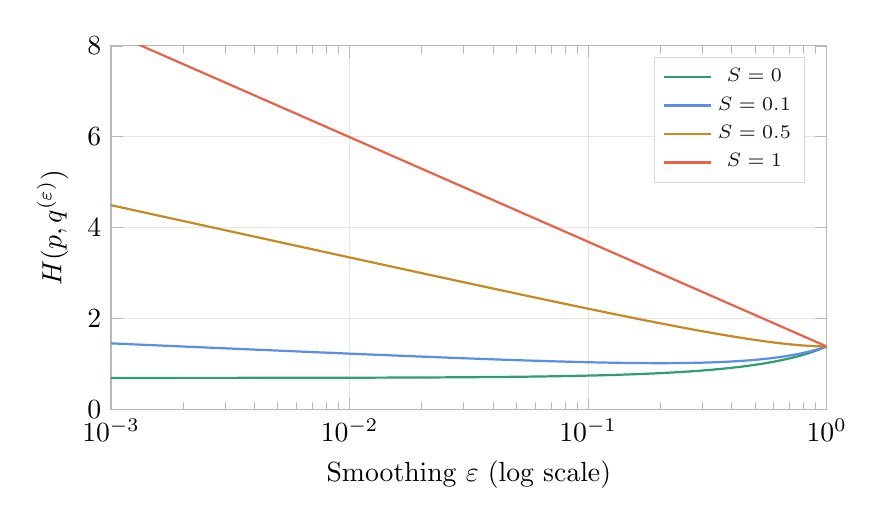
\begin{tikzpicture}
  \begin{axis}[
    width=0.88\textwidth,
    height=6.2cm,
    xlabel={Smoothing $\varepsilon$ (log scale)},
    ylabel={$H(p,q^{(\varepsilon)})$},
    xmin=0.001, xmax=1,
    ymin=0, ymax=8,
    xmode=log,
    grid=major,
    grid style={gray!20},
    axis line style={gray!55},
    tick style={gray!55},
    legend pos=north east,
    legend style={font=\scriptsize,fill=white,fill opacity=0.92,draw=gray!30},
  ]
    \addplot[accentgreen,thick,domain=0.001:1,samples=200]
      {-ln(0.5-0.25*x)};
    \addlegendentry{$S=0$}

    \addplot[accentblue,thick,domain=0.001:1,samples=200]
      {-0.9*ln(0.5-0.25*x)-0.1*ln(0.25*x)};
    \addlegendentry{$S=0.1$}

    \addplot[gold,thick,domain=0.001:1,samples=200]
      {-0.5*ln(0.5-0.25*x)-0.5*ln(0.25*x)};
    \addlegendentry{$S=0.5$}

    \addplot[accent,thick,domain=0.001:1,samples=200]
      {-ln(0.25*x)};
    \addlegendentry{$S=1$}
  \end{axis}
\end{tikzpicture}
\caption{Uniform smoothing for explicit distributions on four symbols.
The coefficient of $-\log\varepsilon$ is the violating mass $S$.
At $\varepsilon=1$, every smoothed distribution is uniform, so every curve equals $\log4$.}
\label{fig:uniform-smoothing}
\end{figure}

\section{Probability coordinates, simplex directions, and logits}
\label{sec:gradients}

Boundary blow-up depends on the coordinate system in which a model is differentiated.

\begin{theorem}[Three differential views of cross-entropy]
\label{thm:gradients}
Fix $p\in\simplex$ and let $q$ lie in the interior of $\simplex$.
\begin{enumerate}[label=(\alph*)]
  \item The ambient probability-coordinate gradient is
  \[
    \nabla_q H(p,q)
    = \left(-\frac{p_i}{q_i}\right)_{i=1}^n.
  \]
  \item For every tangent direction $v\in\mathbb R^n$ with $\sum_i v_i=0$,
  \[
    D H(p,q)[v]
    = -\sum_{i=1}^n\frac{p_i}{q_i}v_i.
  \]
  \item If $q=\operatorname{softmax}(z)$, then
  \begin{align}
    \nabla_z H(p,\operatorname{softmax}(z)) &= q-p, \\
    \nabla_z^2 H(p,\operatorname{softmax}(z))
      &= \operatorname{diag}(q)-qq^\top.
  \end{align}
  In particular, every logit-gradient coordinate lies in $[-1,1]$, and the Hessian is positive semidefinite.
\end{enumerate}
\end{theorem}

\begin{proof}
Parts (a) and (b) follow by differentiating $-\sum_i p_i\log q_i$ in ambient coordinates and along the curve $q+tv$.
For part (c), the softmax Jacobian is
\[
  \frac{\partial q_j}{\partial z_i}=q_j(\mathbf 1\{i=j\}-q_i).
\]
The chain rule gives $\partial H/\partial z_i=q_i-p_i$.
Differentiating once more yields $\operatorname{diag}(q)-qq^\top$, the covariance matrix of a categorical variable with law $q$, hence positive semidefinite.
\end{proof}

The ambient gradient may diverge while the logit gradient stays bounded.
This is not a contradiction: the softmax Jacobian degenerates near the boundary and cancels the $1/q_i$ factor.

\begin{proposition}[Strict propriety and softmax attainability]
\label{prop:proper}
For every $p,q\in\simplex$,
\[
  H(p,q)\ge H(p),
\]
with equality if and only if $q=p$.
Hence $q=p$ is the unique minimiser over the closed simplex.
If $q=\operatorname{softmax}(z)$ with finite $z$, this minimiser is attained if and only if $p$ has full support.
When $p$ has a zero coordinate, the infimum $H(p)$ is approached only as the corresponding logit differences tend to $-\infty$.
\end{proposition}

\begin{proof}
By~\eqref{eq:ce-kl}, it suffices to use Gibbs' inequality $\KL(p\|q)\ge0$, with equality exactly when $p=q$.
A finite softmax vector has full support.
If $p$ has full support, $z_i=\log p_i+c$ gives $\operatorname{softmax}(z)=p$.
If $p$ has a zero coordinate, no finite softmax vector equals $p$, although a sequence of logits can send the corresponding probabilities to zero while the remaining probabilities converge to $p$.
\end{proof}

Proposition~\ref{prop:proper} also blocks a common coordinatewise fallacy.
A summand with $p_i=0$ contributes zero, but increasing $q_i$ is not free on the simplex: it displaces mass from other coordinates.
In logits, its gradient is $q_i>0$, so gradient descent pushes it downward.

\begin{figure}[ht]
\centering
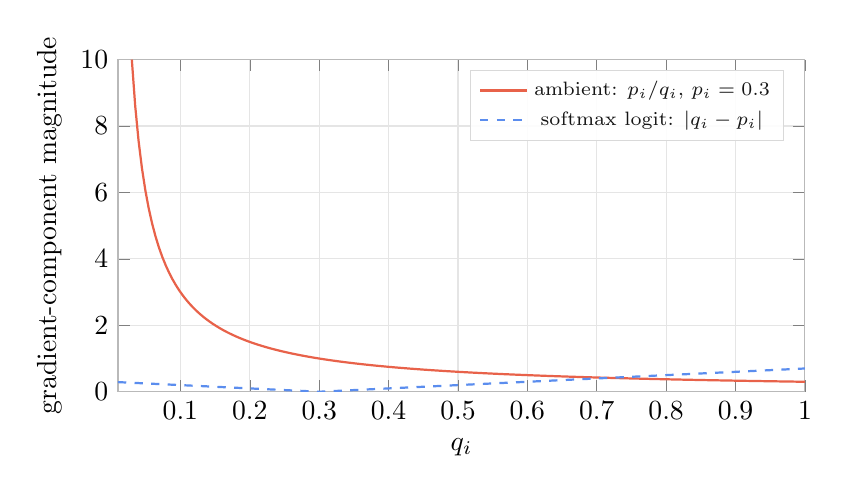
\begin{tikzpicture}
  \begin{axis}[
    width=0.85\textwidth,
    height=5.8cm,
    xlabel={$q_i$},
    ylabel={gradient-component magnitude},
    xmin=0.01, xmax=1,
    ymin=0, ymax=10,
    grid=major,
    grid style={gray!20},
    axis line style={gray!55},
    legend pos=north east,
    legend style={font=\scriptsize,fill=white,fill opacity=0.92,draw=gray!30},
  ]
    \addplot[accent,thick,domain=0.03:1,samples=200] {0.3/x};
    \addlegendentry{ambient: $p_i/q_i$, $p_i=0.3$}
    \addplot[accentblue,thick,dashed,domain=0.01:1,samples=200] {abs(x-0.3)};
    \addlegendentry{softmax logit: $|q_i-p_i|$}
  \end{axis}
\end{tikzpicture}
\caption{The same loss has an unbounded derivative in direct probability coordinates and a bounded derivative through softmax logits.}
\label{fig:gradient-coordinates}
\end{figure}

\section{Finite-temperature contrastive softmax}
\label{sec:contrastive}

Contrastive objectives such as InfoNCE and CLIP apply cross-entropy to a distribution over pair labels obtained from similarities~\cite{oord2018infonce,radford2021clip,chen2020simclr}.
That distribution is not the distribution of embeddings themselves.

Consider a row of $N$ similarities $s_{i1},\dots,s_{iN}$ with designated match $s_{ii}$ and temperature $\tau>0$.
Define
\begin{align}
  Q_{ij}
    &= \frac{\exp(s_{ij}/\tau)}{\sum_{k=1}^N\exp(s_{ik}/\tau)}, \\
  \ell_i
    &= -\log Q_{ii}.
\end{align}
For cosine similarities, $s_{ij}\in[-1,1]$.

\begin{theorem}[No support singularity at finite temperature]
\label{thm:contrastive-finite}
Let $N\ge2$, $\tau>0$, and $s_{ij}\in[-1,1]$.
Then:
\begin{enumerate}[label=(\alph*)]
  \item $Q_{ij}>0$ for every $i,j$, so $\ell_i$ is finite;
  \item
  \begin{equation}
    \log\!\left(1+(N-1)e^{-2/\tau}\right)
    \le \ell_i
    \le
    \log\!\left(1+(N-1)e^{2/\tau}\right);
    \label{eq:contrastive-bounds}
  \end{equation}
  \item
  \begin{equation}
    \frac{\partial\ell_i}{\partial s_{ij}}
    = \frac{Q_{ij}-\mathbf1\{i=j\}}{\tau},
    \qquad
    \left|\frac{\partial\ell_i}{\partial s_{ij}}\right|
    \le\frac1\tau.
    \label{eq:contrastive-gradient}
  \end{equation}
\end{enumerate}
Thus neither the loss nor its similarity gradients have a support singularity at exact orthogonality when $\tau$ is fixed and positive.
\end{theorem}

\begin{proof}
Exponentials of finite numbers are strictly positive, proving (a).
Rewrite
\[
  \ell_i
  = \log\!\left(
      1+\sum_{j\ne i}
      \exp\!\left(\frac{s_{ij}-s_{ii}}{\tau}\right)
    \right).
\]
Since $s_{ij}-s_{ii}\in[-2,2]$, bounding each of the $N-1$ exponentials proves~\eqref{eq:contrastive-bounds}.
Differentiating the log-softmax gives~\eqref{eq:contrastive-gradient}; the bound follows from $0<Q_{ij}<1$.
\end{proof}

\begin{corollary}[Matched pairs with orthogonal negatives]
\label{cor:orthogonal}
If $s_{ii}=1$ and $s_{ij}=0$ for every $j\ne i$, then
\begin{align}
  \ell_i
    &= \log\!\left(1+(N-1)e^{-1/\tau}\right),
    \label{eq:orthogonal-loss} \\
  Q_{ij}
    &= \frac{1}{e^{1/\tau}+N-1}\quad(j\ne i), \\
  \sum_{j\ne i}Q_{ij}
    &= \frac{N-1}{e^{1/\tau}+N-1}.
    \label{eq:negative-mass}
\end{align}
Exact orthogonality is therefore finite.
At fixed geometry and temperature, increasing $N$ raises the total competing negative mass; this is a batch-competition effect, not a support singularity.
\end{corollary}

\begin{proof}
Substitute the stated similarities into the definitions and factor $e^{1/\tau}$ from the denominator.
\end{proof}

\begin{corollary}[How a softmax probability can approach zero]
\label{cor:zero-limit}
For bounded cosine similarities, a contrastive softmax probability can approach zero only through a singular parameter limit, such as $\tau\to0^+$ with a nonmaximal similarity, or through an unbounded logit transformation.
It cannot equal zero at finite positive temperature.
\end{corollary}

This distinction matters when interpreting large batches.
Large batches offer more negatives and increase the chance of hard negatives; they also alter the softmax denominator and estimator variance.
Those mechanisms have been studied empirically and theoretically~\cite{chen2020simclr,ash2022negatives,huang2023modelaware,koromilas2024bridging}.
Equation~\eqref{eq:negative-mass} isolates one elementary denominator effect without attributing it to a nonexistent zero-probability boundary.

\section{Consequences and limits}
\label{sec:discussion}

\subsection{Support mismatch is not geometric separation}

For nonnegative vectors, $p^\top q=0$ is equivalent to disjoint support.
This is a valid algebraic analogy with orthogonality.
It should not be confused with statistical independence, and it does not make $\KL$ a metric.
Relative entropy is asymmetric and extended-real-valued.

Embedding distributions introduce an additional distinction.
Two modalities may occupy separated regions of a sphere, but the CLIP loss is cross-entropy over pair labels computed from finite similarities.
Theorem~\ref{thm:contrastive-finite} shows that separated or orthogonal embeddings do not by themselves create a support violation in that label distribution.
Temperature-dependent repulsion and initialization geometry remain plausible explanations of modality gaps~\cite{liang2022modality,mager2026modality}; they are simply different mechanisms.

\subsection{Coordinatewise asymmetry is not an overcoverage theorem}

The identities
\[
  -p_i\log0=+\infty\quad(p_i>0),
  \qquad
  -0\log q_i=0
\]
are exact.
They do not imply that adding mass to impossible outcomes is globally free.
The simplex couples all coordinates, Proposition~\ref{prop:proper} identifies $q=p$ as the unique optimum, and Theorem~\ref{thm:gradients} gives the positive logit gradient $q_i$ on a zero-target coordinate.
Any claim connecting cross-entropy to hallucination therefore requires a model-specific account of misspecification, decoding, regularisation, or data uncertainty; it does not follow from the summand identity alone.

\subsection{Three different boundary phenomena}

The results suggest a clean taxonomy:
\begin{enumerate}[label=(\roman*)]
  \item \textbf{Support singularity:} $q_i=0<p_i$, giving extended-real loss $+\infty$.
  \item \textbf{Parameter singularity:} a limit such as $\tau\to0^+$ or an unbounded logit gap, potentially sending softmax probabilities to zero.
  \item \textbf{Batch competition:} many finite negative logits contribute through the denominator, changing loss and gradient allocation without any zero probability.
\end{enumerate}
Conflating these phenomena obscures both the mathematics and the optimization behavior.

\section{Conclusion}

Cross-entropy has a sharp support singularity, but the rate at which it is approached is path-dependent.
Uniform smoothing converts the violating mass into the leading coefficient because every uncovered coordinate vanishes with exponent one.
More general paths weight each violating mass by its own vanishing exponent.

The same loss looks different in different coordinates.
Its direct probability derivative can diverge, its simplex derivative must respect coupled directions, and its softmax-logit gradient remains bounded.
For bounded similarities and positive temperature, contrastive softmax has full support and finite gradients; orthogonality is not a singularity.
This separation identifies the genuine mathematical boundary and prevents it from being used as an explanation for phenomena produced by temperature, geometry, or batch composition.

\begin{thebibliography}{20}

\bibitem{cover2006elements}
T.~M. Cover and J.~A. Thomas.
\newblock \emph{Elements of Information Theory}, second edition.
\newblock Wiley, 2006.

\bibitem{csiszar2004information}
I.~Csisz\'ar and P.~C. Shields.
\newblock Information theory and statistics: A tutorial.
\newblock \emph{Foundations and Trends in Communications and Information Theory}, 1(4):417--528, 2004.

\bibitem{oord2018infonce}
A.~van~den~Oord, Y.~Li, and O.~Vinyals.
\newblock Representation learning with contrastive predictive coding.
\newblock \emph{arXiv:1807.03748}, 2018.

\bibitem{radford2021clip}
A.~Radford et al.
\newblock Learning transferable visual models from natural language supervision.
\newblock In \emph{Proceedings of ICML}, 2021.

\bibitem{chen2020simclr}
T.~Chen, S.~Kornblith, M.~Norouzi, and G.~Hinton.
\newblock A simple framework for contrastive learning of visual representations.
\newblock In \emph{Proceedings of ICML}, 2020.

\bibitem{liang2022modality}
W.~Liang, Y.~Zhang, Y.~Kwon, S.~Yeung, and J.~Zou.
\newblock Mind the gap: Understanding the modality gap in multi-modal contrastive representation learning.
\newblock In \emph{Advances in Neural Information Processing Systems}, 2022.

\bibitem{mager2026modality}
F.~Mager, H.~Nassar, and L.~K. Hansen.
\newblock On the modality gap and the contrastive loss in multi-modal representation learning.
\newblock \emph{arXiv:2607.10698}, 2026.

\bibitem{ash2022negatives}
J.~T. Ash, S.~Goel, A.~Krishnamurthy, and D.~Misra.
\newblock Investigating the role of negatives in contrastive representation learning.
\newblock In \emph{Proceedings of AISTATS}, 2022.

\bibitem{huang2023modelaware}
Z.~Huang et al.
\newblock Model-aware contrastive learning: Towards escaping the dilemmas.
\newblock In \emph{Proceedings of ICML}, 2023.

\bibitem{koromilas2024bridging}
P.~Koromilas, G.~Bouritsas, T.~Giannakopoulos, M.~Nicolaou, and Y.~Panagakis.
\newblock Bridging mini-batch and asymptotic analysis in contrastive learning: From InfoNCE to kernel-based losses.
\newblock In \emph{Proceedings of ICML}, 2024.

\end{thebibliography}

\end{document}
